\section{Interpolatory Reduced Order Modeling}

\subsection{Projection Based ROM}

\begin{frame}{Projection Based ROM}
    To compute the reduced order model ${\bf \widehat{H}}(s)$, need to compute projection matrices ${\bf V}, {\bf W} \in \real^{n \times r}$ with $r << n$ such that:
\begin{align*}
    {\bf \widehat{A} } & = {\bf W^{T}} {\bf A} {\bf V} \\
    {\bf \widehat{b} } & = {\bf W^{T}} {\bf b} \\
    {\bf \widehat{c}}^T & = {\bf c}^T {\bf V} \\
    {\bf \widehat{E} } & = {\bf W^{T}} {\bf E} {\bf V}\\
    {\bf \widehat{H}}(s) & = {\bf \widehat{c}}^T \big( s{\bf \widehat{E}}-{\bf \widehat{A}} \big)^{-1} {\bf \widehat{b}} + {\bf \widehat{d}} 
\end{align*}
\\
Given a set of training frequencies $\{\sigma_1, \dots \sigma_r\} \subset \mathbb{I}$, want to find ${\bf V}, {\bf W}$ such that ${\bf H}(\sigma) = {\bf \widehat H}(\sigma)$ for all the training frequencies\\
\bigskip
How to compute ${\bf V}$ and ${\bf W}$?
    
\end{frame}
%%%%%%%%%%%%%%%%%%%%%%%%%%%%%%%%%%%%%%%%%%%%%%%%%%%%%%%%%%%%%%%%%%%%%%
\begin{frame}{Projection Based ROM}
\begin{theorem}
Let \(\sigma \in \mathbb{C}\) be such that \(\big(\sigma{\bf E}-{\bf A} \big)\) and \(\big(\sigma{\bf \widehat E}-{\bf \widehat A} \big)\) are non-singular. Also, let \({\bf V},{\bf W} \in \mathbb{C}^{n \times r}\) have full rank. Then,\\
\bigskip
\begin{enumerate}
    \item <1-> If \(\big( \sigma{\bf E}-{\bf A} \big)^{-1}{\bf b} \in \mathcal{R}\big({\bf V}\big) \), then \({\bf H}(\sigma) = {\bf \widehat{H}}(\sigma)\)
    \item <1-> If \(\big( \sigma{\bf E}^T-{\bf A}^T \big)^{-1} {\bf c} \in \mathcal{R}\big({\bf W}\big) \), then \({\bf H}(\sigma) = {\bf \widehat{H}}(\sigma)\)
    \item If (1) and (2) hold, then \({\bf H}'(\sigma) = {\bf \widehat H}'(\sigma)\)
\end{enumerate}

\end{theorem} 
\noindent

\end{frame}
%%%%%%%%%%%%%%%%%%%%%%%%%%%%%%%%%%%%%%%%%%%%%%%%%%%%%%%%%%%%%%%%

\begin{frame}{Proof of Interpolation Property}

Assume \(\big( \sigma{\bf E}-{\bf A} \big)^{-1}{\bf b} \in \mathcal{R}\big({\bf V}\big) \)\\

\bigskip

Define:
\begin{align*}
    \mathbb{P}(s) & = {\bf V} \Big( s{\bf E-A} \Big)^{-1} {\bf W^{T}} \Big( s{\bf E-A} \Big)\\
    \mathbb{Q}(s) & = \Big( s{\bf E-A} \Big) {\bf V} \Big( s{\bf E-A} \Big)^{-1} {\bf W^{T}}
\end{align*}
\\
\bigskip
\(\mathbb{P}(s)^2 =\mathbb{P}(s)\) and \(\mathbb{Q}(s)^2 = \mathbb{Q}(s) \implies \mathbb{P}(s)\) and \(\mathbb{Q}(s)\) are projections.
\\
\bigskip
Also, make note that \( \mathcal{R}\big( {\bf V} \big) =  \mathcal{R}\big( \mathbb{P}(\sigma) \big)  \) and \(\mathcal{R}\big({\bf W}\big) = \mathcal{R}\big({\bf I - \mathbb{Q}(\sigma)}\big) \).

\end{frame}

%%%%%%%%%%%%%%%%%%%%%%%%%%%%%%%%%%%%%%%%%%%%%%%%%%%%%%%%%%%%%%%%%%%%%%%%%%%%%%%%%%%%%%%%%%%%%%%%%%%%%%%%%%%%%%%%%%

\begin{frame}{Proof of Interpolation Property}
Consider the identity:
$$
    {\bf H}(s) -{\bf \widehat{H}}(s) = 
    {\bf c}^T \Big( s{\bf E-A} \Big)^{-1} \Big( {\bf I} - \mathbb{Q}(s) \Big) \Big( s{\bf E-A} \Big) \Big( {\bf I} - \mathbb{P}(s) \Big) \Big( s{\bf E-A} \Big)^{-1} {\bf b}
$$
\\


Evaluate at \(\sigma\), to get:
$$
    {\bf H}(s) -{\bf \widehat{H}}(s) = \dots \Big( {\bf I} - \mathbb{P}(\sigma)\Big) \Big( \sigma {\bf E-A} \Big)^{-1} {\bf b}
$$
\\
By assumption, \(\Big( \sigma {\bf E-A} \Big)^{-1} {\bf b} \in \mathcal{R}\big({\bf V}\big) \) or \( \in \mathcal{N}\big( {\bf I} - \mathbb{P}(\sigma) \big)\)\\
\bigskip
So:
$$ {\bf H}(\sigma) -{\bf \widehat{H}}(\sigma)  = 0 \implies {\bf H}(\sigma)  = {\bf \widehat{H}}(\sigma)
$$\\
\bigskip
Proof of part (2) follows similarly.    
\end{frame}

%%%%%%%%%%%%%%%%%%%%%%%%%%%%%%%%%%%%%%%%%%%%%%%%%%
\begin{frame}{Proof of Interpolation Property}

Assume parts (1) and (2) of the theorem hold\\

\bigskip

Consider the identity from before:
$$
    {\bf H}(s) -{\bf \widehat{H}}(s) = 
    {\bf c}^T \Big( s{\bf E-A} \Big)^{-1} \Big( {\bf I} - \mathbb{Q}(s) \Big) \Big( s{\bf E-A} \Big) \Big( {\bf I} - \mathbb{P}(s) \Big) \Big( s{\bf E-A} \Big)^{-1} {\bf b}
$$

Evaluate at $s = \sigma + \epsilon$:

$${\bf H}(\sigma + \epsilon) -{\bf \widehat{H}}(\sigma + \epsilon) = \mathcal{O}(\epsilon^2)$$

Since ${\bf H}(\sigma) = {\bf \widehat H}(\sigma)$ by the assumption,

$$\lim_{\epsilon \to 0} \frac{1}{\epsilon}\Big({\bf H}(\sigma + \epsilon) - {\bf H}(\sigma)\Big) - \frac{1}{\epsilon}\Big({\bf \widehat H}(\sigma + \epsilon) - {\bf \widehat H}(\sigma)\Big) = 0$$
which proves part (3) of the theorem.
\end{frame}
%%%%%%%%%%%%%%%%%%%%%%%%%%%%%%%%%%%%%%%%%%%%
\begin{frame}{Projection Matrix Generation}
Choose a list of interpolation frequencies, \([\sigma_1,\sigma_2, ... , \sigma_r]\).\\
\bigskip
Then let us construct the projection matrices and as follows:
\begin{align*}
    {\bf V} & = \Big[ \big( \sigma_1{\bf E}-{\bf A} \big)^{-1}{\bf b}, \dots, \big( \sigma_r{\bf I}-{\bf A} \big)^{-1}{\bf E} \Big] \\
    {\bf W} & = \Big[ \big( \sigma_1{\bf E}^T-{\bf A}^T \big)^{-1} {\bf c}, \dots, \big( \sigma_r{\bf E}^T-{\bf A}^T \big)^{-1} {\bf c} \Big] \\ 
\end{align*}
\end{frame}
%%%%%%%%%%%%%%%%%%%%%%%%%%%%%%%%%%%%%%%%%%%%%%%%%%%%%%%%%%%%%%%%%%%%%%%%%%%%%%%%%%%%%%%%%%%%%%%%%%%%
\begin{frame}{Projection ROM Performance}
\centering
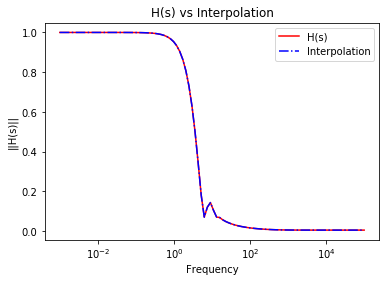
\includegraphics[width=5cm, height= 4cm]{figures/1D_proj.png}
\bigskip
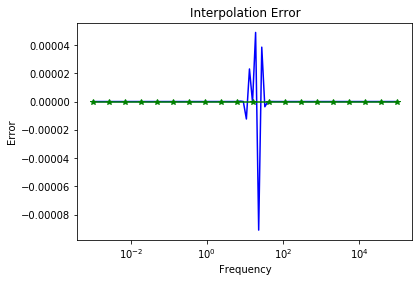
\includegraphics[width=5cm, height=4cm]{figures/1D_proj_err.png}
    
\end{frame}
%%%%%%%%%%%%%%%%%%%%%%%%%%%%%%%%%%%%%%%
\begin{frame}{Projection ROM: Complex to Real}
Since \(\sigma_j\) is complex, \({\bf V}\) and \({\bf W} \in \mathbb{C}\).
\\
The original problem is in the time domain.
\bigskip
\begin{itemize}
    \item <1->Need  real matrices $\bf \widehat A$, $\bf \widehat b$, $\bf \widehat c$, $\bf \widehat d$, and $\bf \widehat E$ \\
    \item <1-> To get \({\bf A} \in \real^{n \times n}, {\bf b} \in \real^{n}\), etc., need real valued {\bf V},{\bf W}
\end{itemize}
\bigskip
\begin{itemize}
    \item <1-> Problem:
    \begin{itemize}
        \item How do we retain the info in {\bf V},{\bf W}?
    \end{itemize}
\end{itemize}
\bigskip
Split into their real and imaginary parts?
\end{frame}



%%%%%%%%%%%%%%%%%%%%%%%%%%%%%%%%%%%%%%%

\begin{frame}{Projection ROM: Complex to Real}
\begin{itemize}
    \item <1-> Split into real and imaginary parts:
\end{itemize}
 Let $\mathbf{V} = \mathbf{V_a} + i \mathbf{V_b}$ and $\mathbf W = \mathbf W_a + i \mathbf W_b$.
\\
\bigskip
Choose $\bf V_{real} = \left[V_a V_b\right]$ and $\bf W_{real} = \left[W_a W_b\right]$.
\\
\bigskip

\begin{itemize}
    \item Problem:
    \begin{itemize}
        \item {\bf V},{\bf W} may be singular
    \end{itemize}
\end{itemize}
\bigskip
Solution? SVD!
\end{frame}
%%%%%%%%%%%%%%%%%%%%%%%%%%%%55
\begin{frame}{Projection ROM: Complex to Real}
SVD purpose = 
\begin{itemize}
    \item <1->remove dependent information
    \item <1-> ensure non-singularity of \( \Big( \sigma \widehat{{\bf E}} - \widehat{{\bf A}} \Big) \)
\end{itemize}

\bigskip
Let $\bf U_v \Sigma_v V_v^T = \left[V_a V_b\right]$ and $\bf U_w \Sigma_w V_w^T = \left[W_a W_b\right]$.
\\
\bigskip
Given a tolerance for the normalized singular values, let \(k_v, k_w =\) number of normalized singular values \(>\) the tolerance.
\bigskip
Set k = max(\(k_v, k_w\)).\\
\bigskip
Then \({\bf V_{real}} = {\bf U_{v_k}}\) and \({\bf W_{real}} = {\bf U_{w_k}}\)
\end{frame}

